% ══════════════════════════════════════════════════════════════════════════════
%  System Design Overview — Cloud Autoscaling Simulator (C++)
%  EECE 2140: Computing Fundamentals for Engineers
%  Northeastern University · Spring 2026
%
%  HOW TO USE ON OVERLEAF:
%  1. Go to https://www.overleaf.com → New Project → Blank Project
%  2. Delete the default main.tex content and paste this entire file
%  3. Click Menu (top-left) → Compiler → select "pdfLaTeX"
%  4. Click Recompile (twice for ToC and cross-references)
%
%  Document content describes the cloud-autoscaling-simulator repository.
% ══════════════════════════════════════════════════════════════════════════════

\documentclass[12pt, a4paper]{article}

% ─── Core Packages ────────────────────────────────────────────────────────────
\usepackage[T1]{fontenc}
\usepackage[utf8]{inputenc}
\usepackage{lmodern}
\usepackage{microtype}
\usepackage[margin=2.5cm, top=2.2cm, bottom=2.5cm, headheight=15pt]{geometry}

% ─── Color & Graphics ─────────────────────────────────────────────────────────
\usepackage[dvipsnames, table, x11names]{xcolor}
\usepackage{graphicx}
\usepackage{tikz}
\usetikzlibrary{shapes.geometric, arrows.meta, positioning, fit,
                calc, decorations.pathreplacing}

% ─── Tables ───────────────────────────────────────────────────────────────────
\usepackage{booktabs}
\usepackage{tabularx}
\usepackage{multirow}
\usepackage{array}
\usepackage{makecell}
\usepackage{longtable}

% ─── Code Listings ────────────────────────────────────────────────────────────
\usepackage{listings}
\usepackage{tcolorbox}
\tcbuselibrary{listings, skins, breakable}

% ─── Layout & Formatting ──────────────────────────────────────────────────────
\usepackage{titlesec}
\usepackage{fancyhdr}
\usepackage{enumitem}
\usepackage{parskip}
\usepackage{setspace}
\usepackage{mdframed}
\usepackage{amsmath}
\usepackage{amssymb}
\usepackage{fontawesome5}   % Requires pdfLaTeX on Overleaf — provides \fa... icons
\usepackage{hyperref}
\hypersetup{
    colorlinks = true,
    linkcolor  = NUNavy,
    urlcolor   = NURed,
    citecolor  = NUNavy,
    pdftitle   = {Cloud Autoscaling Simulator — System Design Overview},
    pdfauthor  = {Wa Fan},
}

% ══════════════════════════════════════════════════════════════════════════════
%  COLOR DEFINITIONS  (Northeastern University palette)
% ══════════════════════════════════════════════════════════════════════════════
\definecolor{NURed}      {RGB}{200,  16,  46}
\definecolor{NUNavy}     {RGB}{  0,  35, 102}
\definecolor{NUNavyL}    {RGB}{ 26,  58, 107}
\definecolor{NULightBlue}{RGB}{173, 204, 223}
\definecolor{NUGray}     {RGB}{210, 210, 210}
\definecolor{NUOffWhite} {RGB}{245, 245, 245}
% Dark code theme
\definecolor{CodeBG}     {RGB}{  5,  15,  30}
\definecolor{CodeText}   {RGB}{171, 178, 191}
\definecolor{CodeGreen}  {RGB}{152, 195, 121}
\definecolor{CodeBlue}   {RGB}{ 97, 175, 239}
\definecolor{CodePurple} {RGB}{198, 120, 221}
\definecolor{CodeOrange} {RGB}{244, 162,  97}
\definecolor{CodeComment}{RGB}{ 92,  99, 112}
\definecolor{CodeRed}    {RGB}{224, 108, 117}
% IPO colors
\definecolor{IPOBlue}    {RGB}{ 21, 101, 192}
\definecolor{IPOGreen}   {RGB}{ 46, 125,  50}
\definecolor{IPOPurple}  {RGB}{106,  27, 154}

% ══════════════════════════════════════════════════════════════════════════════
%  HEADER / FOOTER
% ══════════════════════════════════════════════════════════════════════════════
\pagestyle{fancy}
\fancyhf{}
\renewcommand{\headrule}{%
  {\color{NURed}\hrule width\headwidth height 1.5pt}%
  \vskip 0.8pt%
  {\color{NUNavy!30}\hrule width\headwidth height 0.4pt}%
}
\fancyhead[L]{\small\color{NUNavy}\textbf{EECE 2140} \textcolor{NURed}{$\vert$}
              Computing Fundamentals for Engineers}
\fancyhead[R]{\small\color{NURed}\textbf{Spring 2026}}
\fancyfoot[L]{\small\color{NUNavy}Cloud Autoscaling Simulator}
\fancyfoot[R]{\small\color{NUNavy}\thepage}
\renewcommand{\footrulewidth}{0.4pt}
\renewcommand{\footrule}{{\color{NUGray}\hrule width\headwidth height 0.4pt}}

% ══════════════════════════════════════════════════════════════════════════════
%  SECTION FORMATTING
% ══════════════════════════════════════════════════════════════════════════════
\titleformat{\section}
  {\Large\bfseries\color{NUNavy}}
  {\colorbox{NURed}{\textcolor{white}{\,\thesection\,}}}
  {0.7em}{}
  [\vspace{-4pt}\color{NURed}\rule{\linewidth}{1.5pt}\vspace{2pt}]

\titleformat{\subsection}
  {\large\bfseries\color{NUNavy}}
  {\textcolor{NURed}{\thesubsection}}
  {0.5em}{}
  [\vspace{-3pt}\color{NUGray}\rule{\linewidth}{0.5pt}]

\titleformat{\subsubsection}
  {\normalsize\bfseries\color{NUNavyL}}
  {\textcolor{NURed}{\thesubsubsection}}
  {0.4em}{}

\titlespacing*{\section}      {0pt}{1.4em}{0.6em}
\titlespacing*{\subsection}   {0pt}{1.0em}{0.4em}
\titlespacing*{\subsubsection}{0pt}{0.8em}{0.2em}

% ══════════════════════════════════════════════════════════════════════════════
%  CODE LISTING STYLE
% ══════════════════════════════════════════════════════════════════════════════
\lstdefinestyle{cpp}{
  language         = C++,
  basicstyle       = \ttfamily\footnotesize\color{CodeText},
  backgroundcolor  = \color{CodeBG},
  keywordstyle     = \color{CodePurple}\bfseries,
  commentstyle     = \color{CodeComment}\itshape,
  stringstyle      = \color{CodeGreen},
  numberstyle      = \tiny\color{CodeComment},
  numbers          = left,
  stepnumber       = 1,
  frame            = none,
  breaklines       = true,
  captionpos       = b,
  tabsize          = 4,
  showstringspaces = false,
  keepspaces       = true,
  morekeywords     = {vector,queue,unique_ptr,string,auto,nullptr,bool,float,double,
                      override,struct,class,public,private,virtual,const},
  emph             = {Simulator,Request,Server,ServerCluster,LoadBalancer,AutoScaler,
                      SimMetrics,SimConfig,SimClock,ArrivalMode},
  emphstyle        = \color{CodeOrange},
}
\lstdefinestyle{pseudo}{
  basicstyle       = \ttfamily\footnotesize\color{CodeText},
  backgroundcolor  = \color{CodeBG},
  keywordstyle     = \color{CodePurple}\bfseries,
  commentstyle     = \color{CodeComment}\itshape,
  morekeywords     = {FOR,IF,ELSE,END,RETURN,FUNCTION,PROGRAM,INPUT,
                      OUTPUT,INITIALIZE,GENERATE,ENQUEUE,DEQUEUE,
                      UPDATE,RECORD,TO,AND,NOT,EMPTY,DELETE,MOD},
  numbers          = left,
  stepnumber       = 1,
  frame            = none,
  breaklines       = true,
  tabsize          = 2,
  showstringspaces = false,
  keepspaces       = true,
}
\lstset{style=cpp}

% ══════════════════════════════════════════════════════════════════════════════
%  CUSTOM TCOLORBOX STYLES
% ══════════════════════════════════════════════════════════════════════════════
\newtcolorbox{funccard}[2][]{
  colback    = NURed!4,
  colframe   = NURed,
  coltitle   = white,
  fonttitle  = \bfseries\small,
  title      = {#2},
  sharp corners,
  breakable, #1
}

\newtcolorbox{infocard}[2][]{
  colback    = NUNavy!5,
  colframe   = NUNavy,
  coltitle   = white,
  fonttitle  = \bfseries\small,
  title      = {#2},
  sharp corners,
  breakable, #1
}

\newtcolorbox{codebox}[2][]{
  colback    = CodeBG,
  colframe   = NURed!60,
  coltitle   = white,
  fonttitle  = \bfseries\small\ttfamily,
  title      = {\faCode\enspace #2},
  sharp corners,
  breakable, #1
}

\newtcolorbox{reqbox}[1][]{
  colback    = NUOffWhite,
  colframe   = NUGray,
  sharp corners,
  breakable, #1
}

% ══════════════════════════════════════════════════════════════════════════════
%  TABLE HELPERS
% ══════════════════════════════════════════════════════════════════════════════
\newcolumntype{L}[1]{>{\raggedright\arraybackslash}p{#1}}
\newcolumntype{C}[1]{>{\centering\arraybackslash}p{#1}}
\newcommand{\tblhdr}[1]{\cellcolor{NUNavy}\textcolor{white}{\textbf{#1}}}
\newcommand{\tblgray}{\rowcolor{NUOffWhite}}
\newcommand{\prvt}{\textcolor{NURed}{\textbf{private}}}
\newcommand{\publ}{\textcolor{OliveGreen}{\textbf{public}}}

% ── Misc helpers ──────────────────────────────────────────────────────────────
\newcommand{\cpp}{\texttt{C++}}
\newcommand{\code}[1]{\texttt{\textcolor{NUNavyL}{#1}}}

% ══════════════════════════════════════════════════════════════════════════════
\begin{document}
% ══════════════════════════════════════════════════════════════════════════════

% ────────────────────────────────────────────────────────────────────────────
%  TITLE PAGE
% ────────────────────────────────────────────────────────────────────────────
\begin{titlepage}
  \thispagestyle{empty}

  % Top red banner
  \begin{tikzpicture}[remember picture, overlay]
    \fill[NURed]   (current page.north west)
                   rectangle ([yshift=-2.2cm] current page.north east);
    \fill[NUNavy]  (current page.south west)
                   rectangle ([yshift=1.8cm] current page.south east);
    % Decorative diamond
    \fill[NURed!25] ([xshift=12.5cm, yshift=-1.1cm] current page.north west)
      --++(1.2,0)--++(0,1.2)--++(-1.2,0)--cycle;
    \fill[NURed!12] ([xshift=12cm, yshift=-0.7cm] current page.north west)
      --++(2,0)--++(0,2)--++(-2,0)--cycle;
  \end{tikzpicture}

  % White text on red banner
  {\color{white}\centering
    \vspace*{0.4cm}
    \textbf{\large Northeastern University}\\[3pt]
    \textbf{\normalsize College of Engineering}\\[3pt]
    \textbf{\normalsize Department of Electrical and Computer Engineering}\\
  }

  \vspace{2.2cm}

  % Course box
  \begin{center}
    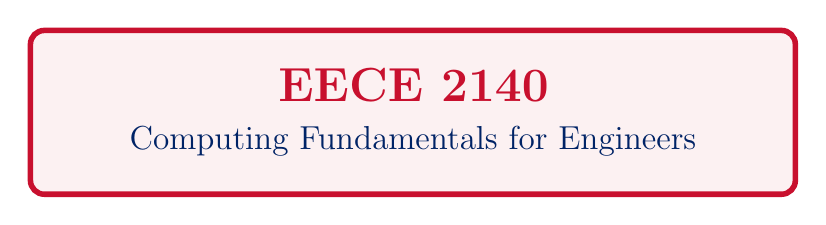
\begin{tikzpicture}
      \node[draw=NURed, line width=2pt, inner sep=14pt,
            rounded corners=5pt, fill=NURed!6] {
        \begin{minipage}{0.72\textwidth}
          \centering
          \textcolor{NURed}{\LARGE\bfseries EECE 2140}\\[5pt]
          \textcolor{NUNavy}{\large Computing Fundamentals for Engineers}
        \end{minipage}
      };
    \end{tikzpicture}
  \end{center}

  \vspace{0.8cm}

  % Main title
  \begin{center}
    {\Huge\bfseries\color{NUNavy} System Design Overview}\\[8pt]
    {\color{NURed}\rule{10cm}{1.5pt}}\\[10pt]
    {\LARGE\bfseries\color{NUNavy} Cloud Autoscaling Simulator}\\[6pt]
    {\large\itshape\color{NUNavyL} A \cpp{} Discrete-Time Simulation Project}
  \end{center}

  \vfill

  % Info block
  \begin{center}
    \setlength{\tabcolsep}{8pt}
    \renewcommand{\arraystretch}{1.4}
    \begin{tabular}{rl}
      \textcolor{NURed}{\faUsers\;\textbf{Author:}}
        & \textbf{Wa Fan}\\[4pt]
      \textcolor{NURed}{\faChalkboard\;\textbf{Instructor:}}
        & Dr.\ Fatema Nafa\\[4pt]
      \textcolor{NURed}{\faCalendarAlt\;\textbf{Semester:}}
        & Spring 2026\\[4pt]
      \textcolor{NURed}{\faGithub\;\textbf{Repository:}}
        & \href{https://github.com/Wallfou/cloud-autoscaling-simulator}{\texttt{github.com/Wallfou/cloud-autoscaling-simulator}}\\
    \end{tabular}
  \end{center}

  \vspace{1.5cm}

  % Footer text over navy bar
  \begin{tikzpicture}[remember picture, overlay]
    \node[anchor=south, yshift=0.55cm, text=white, font=\small]
      at (current page.south)
      {System Design Overview \textbullet\
       EECE 2140 \textbullet\
       Spring 2026};
  \end{tikzpicture}
\end{titlepage}

% ────────────────────────────────────────────────────────────────────────────
\newpage
\tableofcontents
\newpage

% ══════════════════════════════════════════════════════════════════════════════
\section{Project Overview}
% ══════════════════════════════════════════════════════════════════════════════

\begin{infocard}{\faLightbulb\enspace Project Description}
The \textbf{Cloud Autoscaling Simulator} is a \cpp{} program that models a
cloud workload in \emph{discrete time}.
Requests arrive as a Poisson process whose rate can stay constant or vary
over time (smooth sine cycles or alternating burst windows).
Each request waits in a shared FIFO queue, is dispatched by a pluggable
load balancer to a server in an elastic cluster, and is processed for a
random service time.
An \code{AutoScaler} grows or shrinks the fleet using queue-depth thresholds,
cooldown, and optional \emph{provisioning delay} before new instances accept work.
The program reports latency, throughput, utilization-related busy time, and
provisioned server-time so different policies can be compared without using
real infrastructure.
\end{infocard}

\subsection{Motivation}

Cloud autoscaling is a core problem in modern infrastructure.
Understanding how servers respond to changing demand connects directly to how
platforms such as AWS, Azure, and GCP operate at scale, so this project is
based on a real systems problem, not just an academic exercise.
It also came from my interest in distributed systems.
Building the simulation from scratch helped me understand queueing,
resource allocation, and server coordination better than only reading about them.
The project also fit well with object-oriented design, since parts like the
clock, queue, servers, balancers, and scaler could be split into separate
components with clear roles.

\subsection{Project Goals}

\begin{itemize}[leftmargin=1.5em, label=\textcolor{NURed}{\faCheckCircle}]
  \item Design a modular cloud workload simulation framework that models how
    distributed server clusters handle incoming workloads.
  \item Implement request arrival simulation using stochastic traffic patterns,
    including constant, sine-modulated, and burst-style demand.
  \item Implement two load balancing strategies, \code{RoundRobinBalancer} and
    \code{LeastConnectionsBalancer}, and integrate them into the simulation engine.
  \item Implement dynamic autoscaling logic based on queue length, capacity,
    cooldown, and provisioning delay.
  \item Compare results across different configurations in terms of response
    time, wait time, throughput, server utilization, and operational cost.
\end{itemize}

% ══════════════════════════════════════════════════════════════════════════════
\section{Basic Functionalities}
% ══════════════════════════════════════════════════════════════════════════════

This section lists all core functionalities of the simulator together with their
expected inputs, outputs, and contribution to the overall system.

\subsection{Functionality Summary Table}

\renewcommand{\arraystretch}{1.45}
\begin{longtable}{C{0.45cm} L{3.3cm} L{4.3cm} L{2.5cm} L{2.6cm}}
  \toprule
  \tblhdr{\#} & \tblhdr{Functionality} & \tblhdr{Description}
              & \tblhdr{Input}         & \tblhdr{Output} \\
  \midrule
  \endfirsthead
  \toprule
  \tblhdr{\#} & \tblhdr{Functionality} & \tblhdr{Description}
              & \tblhdr{Input}         & \tblhdr{Output} \\
  \midrule
  \endhead
  \bottomrule
  \endlastfoot

  \tblgray
  \textbf{F1} & \textbf{Stochastic arrivals}
    & Each tick samples a Poisson number of new requests using an instantaneous
      rate that may be constant, sine-modulated, or burst on/off.
    & Baseline rate, mode parameters, tick size, RNG seed
    & Request objects enqueued on the shared FIFO \\

  \textbf{F2} & \textbf{Request queue (FIFO)}
    & Holds waiting work between arrival and dispatch; queue length feeds the
      auto-scaler.
    & Enqueue from arrivals; dequeue when a server is chosen
    & Backlog depth, ordered service \\

  \tblgray
  \textbf{F3} & \textbf{Server cluster \& processing}
    & Each Server handles at most one request at a time; the cluster
      can add machines or remove an idle machine.
    & Service-time range, simulation time
    & Busy/idle state, completion events, uptime for metrics \\

  \textbf{F4} & \textbf{Load balancing}
    & RoundRobinBalancer cycles among servers that pass \code{canAcceptWork};
      LeastConnectionsBalancer scores by \code{getActiveConnections()} (0 or 1
      with single-job servers), tie-break lowest id.
    & List of server pointers, current time
    & Target Server* for the next queued request \\

  \tblgray
  \textbf{F5} & \textbf{Auto-scaling}
    & Each tick, subject to cooldown and fleet bounds, the scaler can add a server
      when the queue length reaches the scale-up threshold, or when the fleet is
      non-empty yet no server can accept work while the queue is non-empty
      (all instances still provisioning); it removes an idle server when the
      queue is at or below the scale-down threshold.
    & Thresholds, bounds, cooldown, provisionDelay
    & Updated ServerCluster size over time \\

  \textbf{F6} & \textbf{Metrics \& CLI}
    & Accumulates counts and wait/response totals during the run; provisioned
      time each tick; busy time from server uptimes at shutdown; p95 estimates
      from completed-request samples in \code{finalizeResourceMetrics}; optional
      estimated cost is printed from \code{provisioned time} $\times$
      \code{costPerProvisionedTime} in \texttt{main} (not stored in \code{SimMetrics}).
    & SimConfig via \texttt{main} argument parsing
    & Printed summary after Simulator::run() \\

\end{longtable}

\subsection{Detailed Functionality Descriptions}

\begin{funccard}{\faCloud\enspace F1 — Stochastic arrivals}
\textbf{Description:}
The simulator advances a \code{SimClock} in steps of \code{tickSize}.
Each step, the engine computes an instantaneous Poisson rate from the
selected \code{ArrivalMode} (constant baseline, sine-shaped multiplier, or
alternating burst high/low windows) and draws the number of new requests.
Service demand for each request is uniform in
$[\texttt{serviceTimeMin},\texttt{serviceTimeMax}]$.

\medskip\noindent
\textbf{Input:}  \code{SimConfig} fields for rate, mode, tick, seed. \\
\textbf{Output:} New \code{Request} pointers enqueued on \code{RequestQueue}. \\
\textbf{Contribution:} Provides variable load so queueing, balancing, and scaling matter.
\end{funccard}

\begin{funccard}{\faInbox\enspace F2 — FIFO request queue}
\textbf{Description:}
\code{RequestQueue} wraps \code{std::queue<Request*>} with enqueue, dequeue,
peek, and size helpers.
The queue sits between arrivals and dispatch: the auto-scaler reads only its
length; the simulator drains it when assigning work.

\medskip\noindent
\textbf{Input:}  Pointers to heap-allocated \code{Request} objects. \\
\textbf{Output:} Ordered backlog; length signal for scaling. \\
\textbf{Contribution:} Models waiting work and ties traffic to scaling decisions.
\end{funccard}

\begin{funccard}{\faServer\enspace F3 — Servers and cluster}
\textbf{Description:}
Each \code{Server} tracks whether it is busy, the remaining service time for
the in-flight request, and uptime for accounting.
\code{ServerCluster} owns a \code{std::vector} of servers, supports
\code{addServer(readyTime)} so new machines can have a provisioning delay before
they take traffic, \code{removeServer} on an idle machine, and a per-tick
\code{update} across the fleet.

\medskip\noindent
\textbf{Input:}  Assignments from the simulator; time step from the clock. \\
\textbf{Output:} Completed \code{Request*} when a job finishes; counts of idle,
busy, and accepting servers. \\
\textbf{Contribution:} Represents elastic compute capacity and provisioning lag.
\end{funccard}

\begin{funccard}{\faBalanceScale\enspace F4 — Balancing, scaling, and metrics}
\textbf{Description:}
\code{LoadBalancer} defines \code{selectServer(servers, currentTime)}; concrete
implementations skip busy or still-provisioning machines.
\code{AutoScaler::evaluate} compares queue length to thresholds, detects the
``all servers still provisioning but work is waiting'' case via
\code{acceptingCount}, enforces cooldown and min/max fleet size, and passes
\code{currentTime + provisionDelay} as the new server's ready time on scale-out.
\code{SimMetrics} holds running counters and totals; averages, throughput (via
\code{throughput(duration)}), and sample-based p95 values are derived from those
fields; estimated cost is only computed when printing in \texttt{main}.

\medskip\noindent
\textbf{Input:}  Cluster and queue snapshots each tick; user flags from the CLI. \\
\textbf{Output:} Dispatch decisions, scale events, and end-of-run statistics. \\
\textbf{Contribution:} Turns policy choices into measurable outcomes.
\end{funccard}

% ══════════════════════════════════════════════════════════════════════════════
\section{Object-Oriented Programming (OOP) Design}
% ══════════════════════════════════════════════════════════════════════════════

\subsection{Class Relationship Overview}

The system is split into small types with clear jobs: requests and queueing,
servers and the cluster, balancing and scaling policies, the clock, the
orchestrating \code{Simulator}, and plain \code{SimConfig} / \code{SimMetrics}
data.

\begin{center}
\begin{tikzpicture}[
  box/.style  = {draw=NUNavy, fill=NUOffWhite, rounded corners=4pt,
                 minimum width=3.0cm, minimum height=0.9cm, align=center,
                 font=\small\ttfamily\bfseries, text=NUNavy, drop shadow},
  sbox/.style = {draw=NURed, fill=NURed!6, rounded corners=4pt,
                 minimum width=2.4cm, minimum height=0.8cm, align=center,
                 font=\small\ttfamily\bfseries, text=NURed, drop shadow},
  arr/.style  = {-{Stealth[length=6pt]}, thick, NURed},
  lbl/.style  = {font=\scriptsize\itshape, text=NUNavyL},
]
  \node[box]  (lb)   at (0,   0)    {LoadBalancer};
  \node[box]  (cl)   at (4.2, 0)    {ServerCluster};
  \node[box]  (q)    at (0,  -2.2)  {RequestQueue};
  \node[box]  (sim)  at (4.2,-2.2)  {Simulator};
  \node[sbox] (m)    at (8.4,-2.2)  {SimMetrics};

  \draw[arr] (sim.west)   -- (q.east)
    node[lbl, midway, above=2pt] {owns / steps};
  \draw[arr] (sim.north)  -- (cl.south)
    node[lbl, midway, right=2pt] {owns cluster};
  \draw[arr] (sim.north west)  -- (lb.south east)
    node[lbl, midway, left=1pt] {uses strategy};
  \draw[arr] (lb.east) -- (cl.west)
    node[lbl, midway, above=1pt] {selects server};
  \draw[arr] (sim.east)   -- (m.west)
    node[lbl, midway, above=2pt] {fills metrics};
\end{tikzpicture}
\end{center}

\subsection{OOP Design Table}

\setlength{\tabcolsep}{5pt}
\renewcommand{\arraystretch}{1.40}

\begin{longtable}{L{3cm} L{3.8cm} C{1.4cm} L{4cm} L{3.9cm}}
  \toprule
  \tblhdr{Class} & \tblhdr{Attribute / Method} & \tblhdr{Access}
                 & \tblhdr{Data Type} & \tblhdr{Description} \\
  \midrule
  \endfirsthead
  \toprule
  \tblhdr{Class} & \tblhdr{Attribute / Method} & \tblhdr{Access}
                 & \tblhdr{Data Type} & \tblhdr{Description} \\
  \midrule
  \endhead
  \bottomrule
  \endlastfoot

  % Request
  \multirow{1}{*}{\code{Request}}
    & \code{id\_}                 & \prvt & \code{int}     & Request identifier \\
  \tblgray
    & \code{arrivalTime\_}        & \prvt & \code{double}  & Time the request arrived \\
    & \code{serviceTime\_}        & \prvt & \code{double}  & Total service demand \\
  \tblgray
    & \code{startTime\_}, \code{completionTime\_} & \prvt & \code{double} & Service window \\
    & \code{setStartTime} / \code{setCompletionTime} & \publ & \code{void} & Mutators \\
  \tblgray
    & \code{isComplete()}         & \publ & \code{bool}    & True after processing finishes \\
  \midrule

  % RequestQueue
  \multirow{1}{*}{\code{RequestQueue}}
    & \code{queue\_}              & \prvt & \texttt{std::queue<Request*>} & FIFO backlog \\
  \tblgray
    & \code{enqueue} / \code{dequeue} & \publ & \code{void} / \code{Request*} & Queue ops \\
    & \code{peek} / \code{size}   & \publ & \code{Request*} / \code{int} & Introspection \\
  \tblgray
    & \code{empty()}              & \publ & \code{bool}    & True if no waiting work \\
  \midrule

  % Server
  \multirow{1}{*}{\code{Server}}
    & \code{id\_} / \code{readyTime\_} & \prvt & \code{int}, \code{double} & Identity; accept-after time \\
  \tblgray
    & \code{busy\_}               & \prvt & \code{bool}    & Whether a job is in flight \\
    & \code{currentRequest\_}     & \prvt & \code{Request*}& In-service request (or null) \\
  \tblgray
    & \code{canAcceptWork(t)}     & \publ & \code{bool}    & Idle and past ready time \\
    & \code{assignRequest}        & \publ & \code{void}    & Starts processing a request \\
  \tblgray
    & \code{update(t, dt)}        & \publ & \code{Request*}& Completed request this tick (or null) \\
    & \code{getUptime()}          & \publ & \code{double}  & Busy time for utilization metrics \\
  \midrule

  % ServerCluster
  \multirow{1}{*}{\code{ServerCluster}}
    & \code{servers\_}            & \prvt & \texttt{std::vector<Server*>} & Fleet storage \\
  \tblgray
    & \code{addServer(readyTime)} & \publ & \code{Server*} & Adds capcaity (optional delay) \\
    & \code{removeServer()}       & \publ & \code{bool}    & Removes one idle server \\
  \tblgray
    & \code{acceptingCount(t)}    & \publ & \code{int}     & Servers that can take work now \\
    & \code{update(...)}          & \publ & \texttt{vector<Request*>} & Per-tick completions \\
  \midrule

  % LoadBalancer
  \multirow{1}{*}{\code{LoadBalancer}}
    & \code{selectServer(...)}    & \publ & \code{Server*} & Pure virtual dispatch hook \\
  \tblgray
    & \code{name()}              & \publ & \code{const char*} & Policy label for logs \\
    & virtual destructor          & \publ & ---            & Safe deletion via base pointer \\
  \midrule

  % RoundRobinBalancer
  \multirow{1}{*}{\code{RoundRobin}}
    & \code{lastIndex\_}          & \prvt & \code{int}     & Cyclic scan state \\
  \tblgray
    & \code{selectServer(...)}    & \publ & \code{Server*} & Next eligible server in rotation \\
  \midrule

  % LeastConnectionsBalancer
  \multirow{1}{*}{\code{LeastConnections}}
    & (stateless policy)          & \prvt & ---            & No fields beyond vtable \\
  \tblgray
    & \code{selectServer(...)}    & \publ & \code{Server*} & Min.\ \code{getActiveConnections()} among \code{canAcceptWork}; tie lowest id \\
  \midrule

  % AutoScaler
  \multirow{1}{*}{\code{AutoScaler}}
    & threshold / cooldown fields & \prvt & \code{int}, \code{double} & Scale policy parameters \\
  \tblgray
    & \code{evaluate(cluster, queue, t)} & \publ & \code{void} & Applies scale-out/in rules \\
    & getters for thresholds      & \publ & mixed          & Inspect configuration \\
  \midrule

  % Simulator
  \multirow{1}{*}{\code{Simulator}}
    & \code{config\_}, \code{clock\_} & \prvt & \code{SimConfig}, \code{SimClock} & Time and settings \\
  \tblgray
    & \code{queue\_}, \code{cluster\_} & \prvt & \code{RequestQueue}, \code{ServerCluster} & Core state \\
    & \code{balancer\_}, \code{scaler\_} & \prvt & pointers     & Pluggable policies \\
  \tblgray
    & \code{run()} / \code{step()}& \publ / \prvt & \code{void} & Main loop driver \\
    & \code{getMetrics()}         & \publ & \texttt{const SimMetrics\&} & Result access \\
  \midrule

  % SimConfig
  \multirow{1}{*}{\code{SimConfig}}
    & arrival/scaling fields      & \publ & \code{double}/\code{int} & CLI-populated knobs \\
  \tblgray
    & \code{arrivalMode}          & \publ & \code{ArrivalMode} & Member selecting constant / sine / burst \\
    & \code{costPerProvisionedTime} & \publ & \code{double} & Rate used by \texttt{main} for printed cost \\
  \midrule

  % SimMetrics
  \multirow{1}{*}{\code{SimMetrics}}
    & wait/response totals        & \publ & \code{double} & Accumulated delay \\
  \tblgray
    & \code{totalProvisionedTime} / \code{totalBusyTime} & \publ & \code{double} & Capacity accounting \\
    & \code{avgWaitTime()} etc.   & \publ & \code{double} & Simple derived statistics \\
  \tblgray
    & \code{throughput(duration)} & \publ & \code{double} & Completed work per time \\

\end{longtable}

\subsection{Key OOP Requirements}

\begin{reqbox}
\begin{itemize}[label=\textcolor{NURed}{\faCheckCircle}, leftmargin=1.5em]
  \item \textbf{Multiple cohesive classes:}
    Requests, queue, servers, cluster, simulator, scaler, clock, and metrics
    are separate types instead of one big file.
  \item \textbf{Private state:} Implementation details such as the STL
    \code{queue} inside \code{RequestQueue} stay behind public interfaces.
  \item \textbf{Polymorphic load balancing:}
    \code{LoadBalancer} exposes a virtual \code{selectServer} contract; concrete
    balancers plug into the same \code{Simulator} loop.
  \item \textbf{Enumerated traffic modes:}
    \code{ArrivalMode} is an \code{enum class} for constant, sine, and burst
    arrival patterns.
  \item \textbf{Ownership model:} The simulator owns the lifecycle of requests
    it allocates while the queue and servers hold non-owning pointers, which
    makes the responsibilities clear.
\end{itemize}
\end{reqbox}

% ══════════════════════════════════════════════════════════════════════════════
\section{System Overview — Input, Process, Output}
% ══════════════════════════════════════════════════════════════════════════════

\subsection{High-Level Description}

The simulator follows a basic \textbf{Input $\to$ Process $\to$ Output}
model. Inputs are mostly supplied at startup through \texttt{main}'s
command-line flags (stored in \code{SimConfig}); the process is a discrete
time-stepped loop inside \code{Simulator::run}; outputs are printed after the
run completes.

\subsection{IPO Diagram}

\begin{center}
    \includegraphics[width=1\textwidth]{IPO_DIAGRAM.png}
\end{center}

\subsection{Detailed Step Descriptions}

\subsubsection{Input}
\begin{itemize}[label=\textcolor{IPOBlue}{$\rightarrow$}]
  \item \textbf{Simulation clock:} Tick size and total duration.
  \item \textbf{Cluster:} Initial server count, minimum and maximum cluster size,
    and optional provisioning delay before new servers accept traffic.
  \item \textbf{Workload:} Arrival mode: constant, sine, or burst. Baseline
    Poisson rate and mode-specific parameters.
  \item \textbf{Service times:} Uniform range
    $[\texttt{serviceTimeMin},\texttt{serviceTimeMax}]$ for each request.
  \item \textbf{Autoscaling:} Scale-up and scale-down queue thresholds and
    cooldown between scaling actions.
  \item \textbf{Routing:} Load balancer policy, such as round-robin or
    least-connections.
  \item \textbf{Stochasticity and cost:} RNG seed and optional cost rate on
    provisioned server-time.
\end{itemize}

\subsubsection{Process}

At each discrete tick (length \code{tickSize}):

\begin{enumerate}[label=\textcolor{NURed}{\textbf{Step \arabic*.}},
                  leftmargin=2.2em]
  \item \textbf{Generate arrivals.} The instantaneous rate $\lambda(t)$ depends
    on the selected arrival mode. The simulator samples Poisson counts, creates
    \code{Request} objects with random service times, and enqueues them.
  \item \textbf{Auto-scale.} \code{AutoScaler::evaluate} inspects queue depth and
    \code{acceptingCount} (servers that pass \code{canAcceptWork}), then may add
    or remove servers subject to thresholds, bounds, cooldown, and provisioning
    delay.
  \item \textbf{Dispatch.} While the queue is non-empty and some server can take
    work, the load balancer selects an eligible server and the front request is
    assigned from the global FIFO queue.
  \item \textbf{Serve and complete.} \code{ServerCluster::update} advances work,
    completes requests whose service time has finished, and returns them for
    metric collection.
  \item \textbf{Accumulate resources.} Provisioned time increases with cluster
    size times \code{tickSize}, and request completions update wait and response
    statistics.
\end{enumerate}

\subsubsection{Output}
\begin{itemize}[label=\textcolor{IPOGreen}{$\rightarrow$}]
  \item \textbf{Total and completed requests:} How many arrived and how many finished.
  \item \textbf{Average wait and response time:} Per completed request.
  \item \textbf{p95 wait and respons:} Tail latency for completed requests.
  \item \textbf{Throughput:} Completed requests per unit time over the run.
  \item \textbf{Provisioned and busy time:} Capacity time versus actual processing time.
  \item \textbf{Final server count:} Cluster size at the end of the simulation.
  \item \textbf{Estimated cost:} Printed in \texttt{main} as
    \code{totalProvisionedTime * costPerProvisionedTime} when the cost rate is
    positive (not a field inside \code{SimMetrics}).
\end{itemize}

% ══════════════════════════════════════════════════════════════════════════════
\section{Pseudo Code}
% ══════════════════════════════════════════════════════════════════════════════

\begin{codebox}{Main Simulation Loop}
\begin{lstlisting}[style=pseudo]
PROGRAM CloudAutoscalingSimulator
  INPUT  SimConfig, LoadBalancer strategy
  INITIALIZE Simulator with clock, empty queue, ServerCluster,
            AutoScaler thresholds, RNG for arrivals and service times

  WHILE currentTime < duration:
    t  = clock.currentTime()
    dt = clock.tickSize()

    generateArrivals(t, dt)
    scaler.evaluate(cluster, queue, t)
    dispatchQueuedRequests()
    completed = cluster.update(t + dt, dt)
    collectMetrics(completed)
    accrueProvisionedServerTime(cluster.size() * dt)

    clock.tick()
  END WHILE

  finalizeResourceMetrics()
  OUTPUT  printSummary(metrics)
END PROGRAM
\end{lstlisting}
\end{codebox}

\begin{codebox}{Sub-Function: generateArrivals(t, dt)}
\begin{lstlisting}[style=pseudo]
FUNCTION generateArrivals(t, dt):
  lambda = instantaneousArrivalRate(t)
  n = Poisson(lambda * dt)
  REPEAT n times:
    service = Uniform(serviceMin, serviceMax)
    req = new Request(nextId++, t, service)
    queue.enqueue(req)
    metrics.totalRequests++
  END REPEAT
END FUNCTION
\end{lstlisting}
\end{codebox}

\begin{codebox}{Sub-Function: dispatchQueuedRequests()}
\begin{lstlisting}[style=pseudo]
FUNCTION dispatchQueuedRequests():
  WHILE queue NOT EMPTY:
    server = balancer.selectServer(cluster.servers, currentTime)
    IF server == NULL:
      BREAK
    END IF
    req = queue.dequeue()
    server.assignRequest(req, currentTime)
  END WHILE
END FUNCTION
\end{lstlisting}
\end{codebox}

% ══════════════════════════════════════════════════════════════════════════════
\section{C++ Implementation Highlights}
% ══════════════════════════════════════════════════════════════════════════════

\begin{codebox}{\texttt{Simulator::step()} — Core \cpp{} Implementation}
\begin{lstlisting}
void Simulator::step() {
    double t  = clock_.getTime();
    double dt = clock_.getTickSize();

    generateArrivals(t, dt);

    scaler_.evaluate(cluster_, queue_, t);

    dispatchQueuedRequests();

    std::vector<Request*> completed = cluster_.update(t + dt, dt);
    collectMetrics(completed);

    metrics_.totalProvisionedTime += static_cast<double>(cluster_.size()) * dt;
}
\end{lstlisting}
\end{codebox}

\begin{infocard}{\faCogs\enspace Key Design Decisions}
\begin{enumerate}[label=\textcolor{NURed}{\textbf{D\arabic*.}}, leftmargin=2em]
  \item \textbf{Strategy object for balancing:}
    \code{Simulator} stores a \code{LoadBalancer*} so the same stepping code runs
    with different strategies by swapping the concrete object in
    \texttt{main}.
  \item \textbf{Effective capacity in scaling:}
    The scaler checks how many servers \emph{can accept work now}, not only
    total fleet size, so it can still scale out when the queue is growing but
    new instances are not ready yet.
  \item \textbf{Struct configuration:}
    \code{SimConfig} bundles command line parameters in one place, which keeps
    the experiment setup compact and readable.
  \item \textbf{Metrics separated from control flow:}
    \code{SimMetrics} holds counters and derived statistics while the simulator
    focuses on orchestration and state updates.
\end{enumerate}
\end{infocard}

% ══════════════════════════════════════════════════════════════════════════════
\section{Challenges, Solutions \& Lessons Learned}
% ══════════════════════════════════════════════════════════════════════════════

\subsection{Challenges \& Solutions}
\color{black}

\renewcommand{\arraystretch}{1.5}
\begin{tabularx}{\textwidth}{C{0.4cm} L{4.5cm} X}
  \toprule
  \tblhdr{\#} & \tblhdr{Challenge} & \tblhdr{Solution} \\
  \midrule
  1 & Balancer picked busy servers and dispatch stalled.
    & Centralized \texttt{canAcceptWork(now)} checks inside \code{Server} and
      only exposed eligible machines to \code{selectServer}. \\
  \tblgray
  2 & Scale-out ignored machines still provisioning; backlog grew quickly.
    & Tied scale decisions to \code{acceptingCount(currentTime)} and included
      \code{provisionDelay} on \code{addServer}. \\
  3 & Comparing runs required deterministic traffic.
    & Added a configurable RNG seed so the same workload could be replayed
      across multiple balancer and autoscaler settings. \\
  \bottomrule
\end{tabularx}

\subsection{Lessons Learned}

\begin{itemize}[label=\textcolor{NURed}{\faStar}, leftmargin=1.5em]
  \item \textbf{Threshold-based autoscaling is reactive:} the system responds to
    load after it appears rather than anticipating it, so spikes and first-wave
    lag are visible in bursty or sine-shaped traffic.
  \item \textbf{Cooldown is a tradeoff:} it prevents rapid oscillation, but it
    also slows down how quickly the system can match demand changes.
  \item \textbf{Balancers do not always diverge:} in our logged runs, completion
    counts and average latency often matched between round-robin and
    least-connections under the same seed, while per-server busy time could still
    differ when dispatch order changed which machines stayed active.
\end{itemize}

% ══════════════════════════════════════════════════════════════════════════════
\section{Limitations \& Future Work}
% ══════════════════════════════════════════════════════════════════════════════

\renewcommand{\arraystretch}{1.5}
\begin{tabularx}{\textwidth}{L{4.0cm} X}
  \toprule
  \tblhdr{Current Limitation} & \tblhdr{Proposed Future Extension} \\
  \midrule
  Homogeneous servers and one job per server narrow how much two balancers differ.
    & Introduce heterogeneous servers with different processing speeds or
      capacities so balancer choices have a more meaningful impact. \\
  \tblgray
  Autoscaling relies mostly on queue-length thresholds.
    & Incorporate utilization-based or response-time-based scaling signals for
      a more realistic picture of system health. \\
  \tblgray
  Simple Poisson + uniform service assumptions.
    & Use trace-driven arrivals or heavier-tailed service distributions for
      more realistic workload studies. \\
  Single data centre abstraction.
    & Split traffic across regions with latency penalties and separate
      autoscalers per zone. \\
  \tblgray
  \bottomrule
\end{tabularx}

% ══════════════════════════════════════════════════════════════════════════════
\section{Representative Results}
% ══════════════════════════════════════════════════════════════════════════════

\subsection{Autoscaling Policy Comparison}

\renewcommand{\arraystretch}{1.45}
\begin{tabularx}{\textwidth}{L{2.0cm} L{3.1cm} C{1.5cm} C{1.6cm} C{1.8cm} C{2.1cm} C{1.4cm}}
  \toprule
  \tblhdr{Policy} & \tblhdr{Thresholds (queue length)} & \tblhdr{Cooldown}
  & \tblhdr{Completed} & \tblhdr{Avg Wait} & \tblhdr{Throughput} & \tblhdr{Cost} \\
  \midrule
  Default
    & Scale up $\geq 5$, down $\leq 1$
    & 20 & 2113 & 189.55 & 2.641 & 7.44 \\
  \tblgray
  Aggressive
    & Scale up $\geq 3$, down $\leq 1$
    & 15 & 2151 & 178.63 & 2.689 & 7.58 \\
  Conservative
    & Scale up $\geq 10$, down $\leq 2$
    & 30 & 2027 & 210.78 & 2.534 & 7.152 \\
  \tblgray
  Fast Cooldown
    & Scale up $\geq 5$, down $\leq 1$
    & 8 & 2207 & 163.19 & 2.759 & 7.776 \\
  \bottomrule
\end{tabularx}

\subsection{Result Discussion}

The Fast Cooldown policy gave the best performance overall.
It completed the most requests, had the lowest average wait time, and produced
the highest throughput.
That improvement also came with the highest cost, since faster reactions allowed
the cluster to spin up capacity more often and accumulate more provisioned time.

The Conservative policy was the cheapest, but it also had the weakest
performance.
Because it waited for the queue to grow larger before scaling out, requests
spent longer waiting and fewer requests completed during the run.

The Aggressive policy improved on the default by reacting earlier to
queue buildup, while the Default policy stayed between
aggressive and conservative on the main metrics.

\subsection{Arrival Pattern Behavior}

Across constant, sine, and burst arrival modes, the simulator showed that
threshold-based autoscaling is reactive.
Queue depth often rises first, then the cluster catches up after scale-out.
This lag is especially visible under sine shaped traffic and burst windows,
where demand changes more quickly than the autoscaler can respond.
Cooldown helps prevent oscillation, but it also makes it harder for the system
to instantly match rapid workload changes.

% ══════════════════════════════════════════════════════════════════════════════
\section{GitHub Repository Structure}
% ══════════════════════════════════════════════════════════════════════════════

\begin{codebox}[]{Repository Layout}
\begin{lstlisting}[style=pseudo, numbers=none]
cloud-autoscaling-simulator/
|-- include/
|   |-- Simulator.h
|   |-- SimClock.h
|   |-- Request.h
|   |-- RequestQueue.h
|   |-- Server.h
|   |-- ServerCluster.h
|   |-- LoadBalancer.h
|   |-- AutoScaler.h
|   `-- ...
|-- src/
|   |-- Simulator.cpp
|   |-- main.cpp
|   `-- ...
|-- demo/
|   `-- index.html
|-- experiments/
|   |-- WEEK4_CASES.md
|   `-- results.txt
|-- Makefile
`-- README.md
\end{lstlisting}
\end{codebox}

% ══════════════════════════════════════════════════════════════════════════════
\appendix
\section{Sample Program Output}
% ══════════════════════════════════════════════════════════════════════════════

\begin{codebox}[]{Expected Console Output — End-of-Run Report}
\begin{lstlisting}[style=pseudo, numbers=none]
[Simulator] Starting with balancer: RoundRobin, tick=1, duration=100,
            servers=2, arrival_mode=constant
[Simulator] Done. t=100 completed = 141/213 servers_final = 7

=== Sample run ===
Balancer:           RoundRobin
Arrival mode:       constant
Baseline rate:      2 req/time
Service time:       U[1, 5]
Seed:               42
Autoscale:          queue >= 5 out, queue <= 1 in, cooldown=20
Server bounds:      [1, 10]
Provision delay:    0

=== Results ===
Total requests:     213
Completed requests: 141
Avg wait time:      22.6596
Avg response time:  26.078
p95 wait time:      34
p95 response time:  38
Throughput:         1.41 req/time unit
Provisioned time:   490
Total busy time:    490 (sum of server processing time)
Final servers:      7
Utilization (busy/provisioned): 1
\end{lstlisting}
\end{codebox}

\section{ArrivalMode Enum Definition}

\begin{codebox}[]{\code{Simulator.h} — Arrival Modes (excerpt)}
\begin{lstlisting}
enum class ArrivalMode {
  Constant,
  Sine,
  Burst,
};

struct SimConfig {
  double tickSize = 1.0;
  double duration = 1000.0;
  double arrivalRate = 2.0;
  ArrivalMode arrivalMode = ArrivalMode::Constant;
  // ... remaining fields omitted for brevity ...
};
\end{lstlisting}
\end{codebox}

\end{document}